\chapter{Entwicklung der BMS-Algorithmus}\thispagestyle{fancy}


\section{Einf�hrung in die Batterie Management System}
\large{(Was ist das?, wozu nutzt man?, die Einweisungen, was ist meine Aufgabe?)}


\section{Erstellung eines BMS-Planes}
\large{Die Batterien sollen mit dem BMS-System belegt werden. Daf�r war ein Plan zur Verteilung von BMS Platinen konzipiert. Es waren mehrere Versionen entstanden, wie die Platinen verbunden werden. Wichtige Punkten waren, dass die Kommunikationskabeln nicht l�nger als das festgelegte Maximum werden und dass die Batteriezellen mit dem BMS System verbunden werden. Der Plan sollte �bersichtlich sein, weil es f�r die Orientierung in dem EBU dienen soll. Den Plan habe ich in Microsoft Word erstellt. Ich sollte die Nummerierung von Platinen festlegen. In einen EBU gibt es 16 Trog-Verbunde mit jeweils 5 Tr�gen. Ein Trog hat zwei Zellenbl�cke mit jeweils 6 Zellen. Eine Platine kann Werten von zwei Zellenbl�cken messen. Die Platine reicht aber mit Kabeln nicht �ber einen Trog, das hei�t, dass die BMS die Werten von zwei nebenstehenden Zellenbl�cke messen muss.\\
In der erste Plan habe ich die Verteilung und Nummerierung ausf�hrlich beschreiben (siehe Abbildung \ref{Plan_Trogverbund} und \ref{plan_legende}). \\


\begin{figure}[htbp]
  \centering
     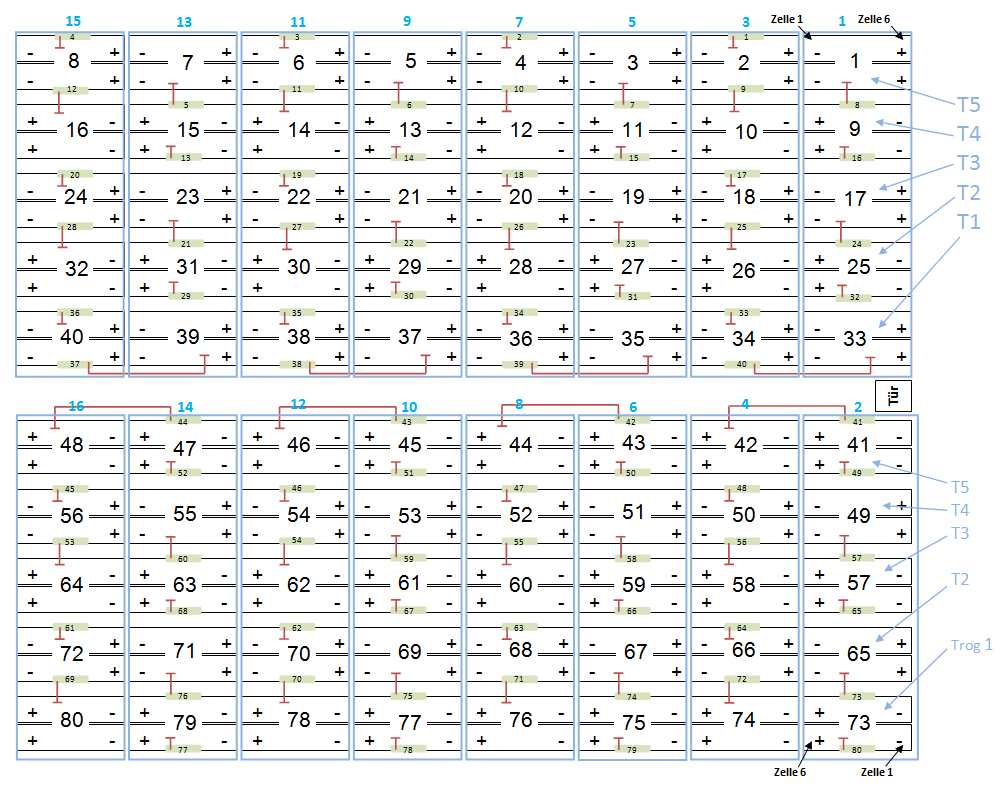
\includegraphics[width=0.99\textwidth]{images/Plan_Trogverbund.png}
  \caption{Plan mit Beschriftung}
  \label{Plan_Trogverbund}
\end{figure}

\begin{figure}[htbp]
  \centering
     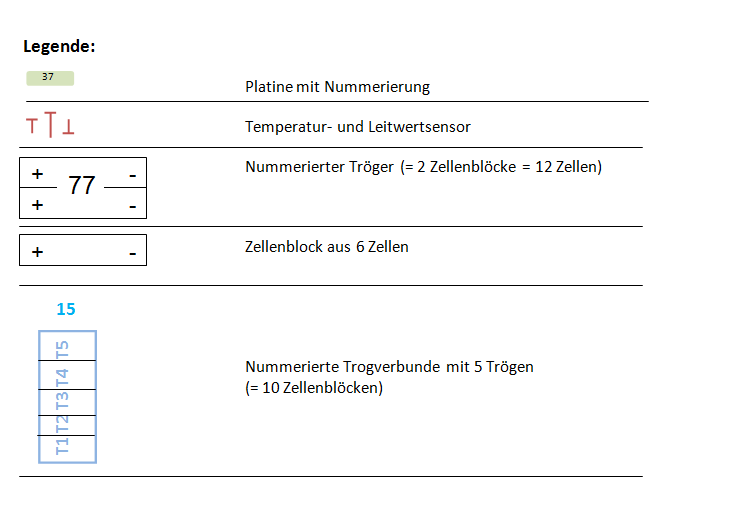
\includegraphics[width=0.6\textwidth]{images/plan_legende.png}
  \caption{Die Legende zum Plan}
  \label{plan_legende}
\end{figure}

\pagebreak
In den zweiten Plan geht es haupts�chlich um das Verkabelung zwischen BMS-Platinen. Die Platinen wurden mit Kommunikationskabeln verbunden. Dies ist mit blau gezeichnet (siehe Abbildung \ref{Montage_plan}).

\begin{figure}[htbp]
  \centering
     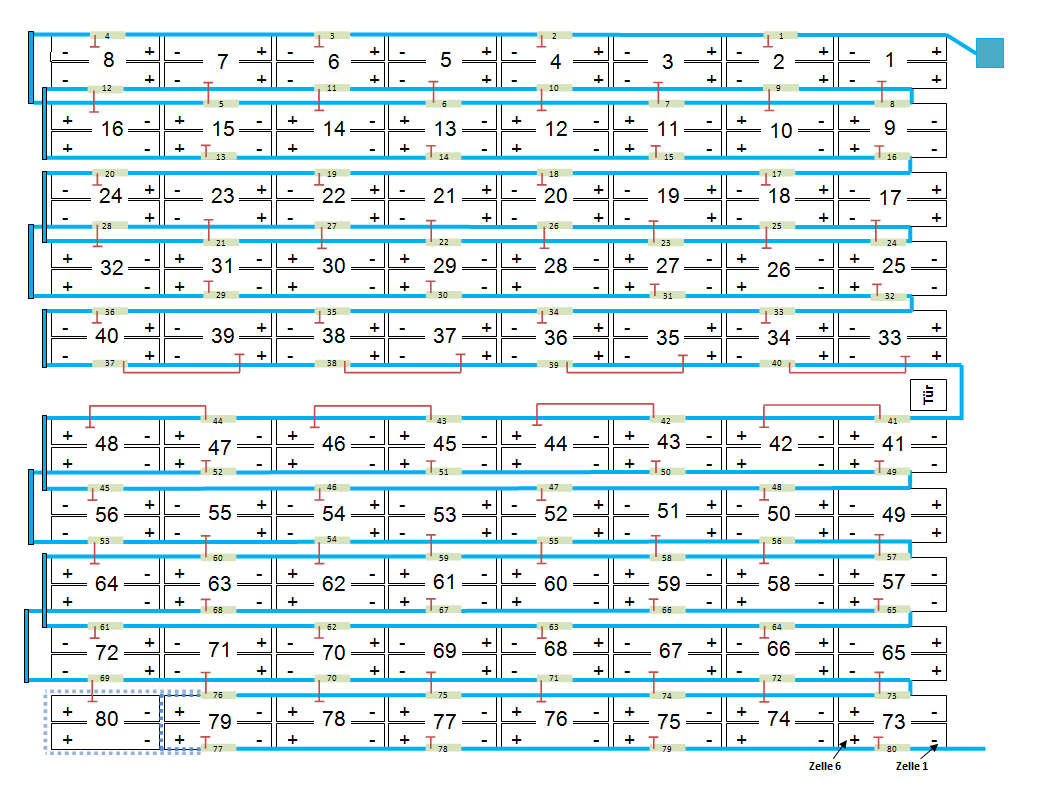
\includegraphics[width=0.9\textwidth]{images/Montage_plan.png}
  \caption{Verkabelung von Platinen}
  \label{Montage_plan}
\end{figure}
\pagebreak


\section{Entwicklung der Algorithmus}
\large{Zu n�chst habe ich paar Tabellen im Excel erstellt. Die erste Tabelle beinhaltet Informationen zur Verteilung von Platinen. Aus dieser Tabelle sollte man schnell die Nummer der Platine auslesen, welche zum Beispiel die Batteriezelle Nummer 5 des Troges 2 des Trog-Verbundes 11 messen wurde (siehe Abbildung \ref{tabelle_excel}). Diese Tabelle dient f�r die bessere Orientierung in einen EBU. \\ 
In der n�chste Tabelle ist der Zusammenhang zwischen eingeladene und festgestellte Werte-Indexen beschrieben. Aus diese Tabelle sollte man zum Beispiel auslesen, dass die Platine Nummer 1 die Indexen 0 bis 14 mit Werten von 5. Trog des 1. und 3. Trog-Verbundes beladet. Die Indexen 0 bis 14 werden mit Werten aufgeladen, aber damit es sortiert wird, muss man die Indexen auf die festgesetzte Indexen aufladen, in diesem Fall wurden es Indexen von 210 bis 215, von 60 bis 65 und drei Indexen 222, 223 und 224 (siehe Abbildung \ref{example_tabelle_indexing}). Die Visualisierung wird die festgelegte Anordnung anzeigen.\\ 	
	
\begin{figure}[htbp]
  \centering
     \subfigure[Tabelle mit Tr�gen in Reihe]{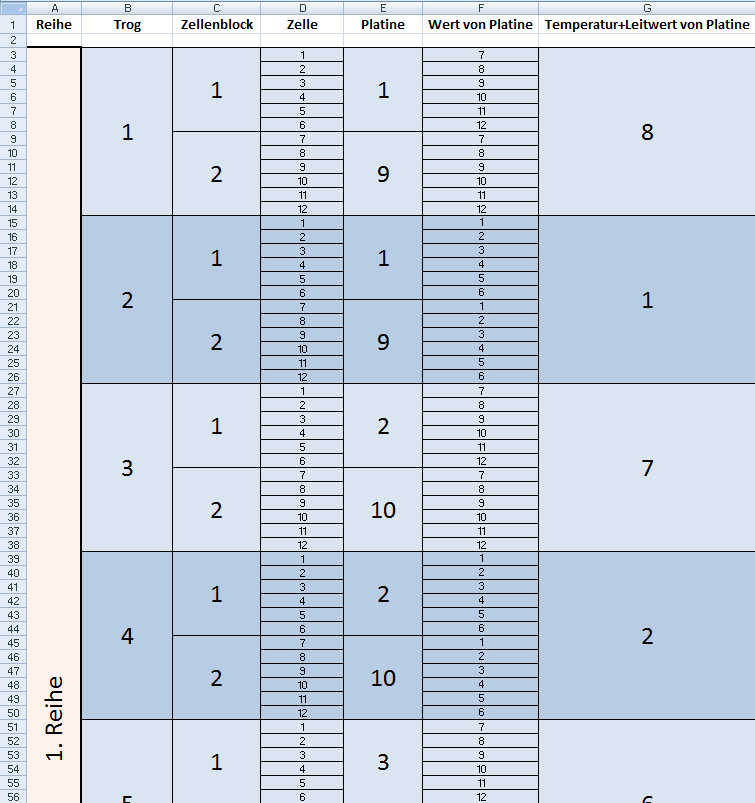
\includegraphics[width=0.42\textwidth]{images/example_tabelle_excel.png}}
			\hspace{1mm}
			\subfigure[Tabelle mit Tr�gen in Trog-Verbunde Reihenordnung]{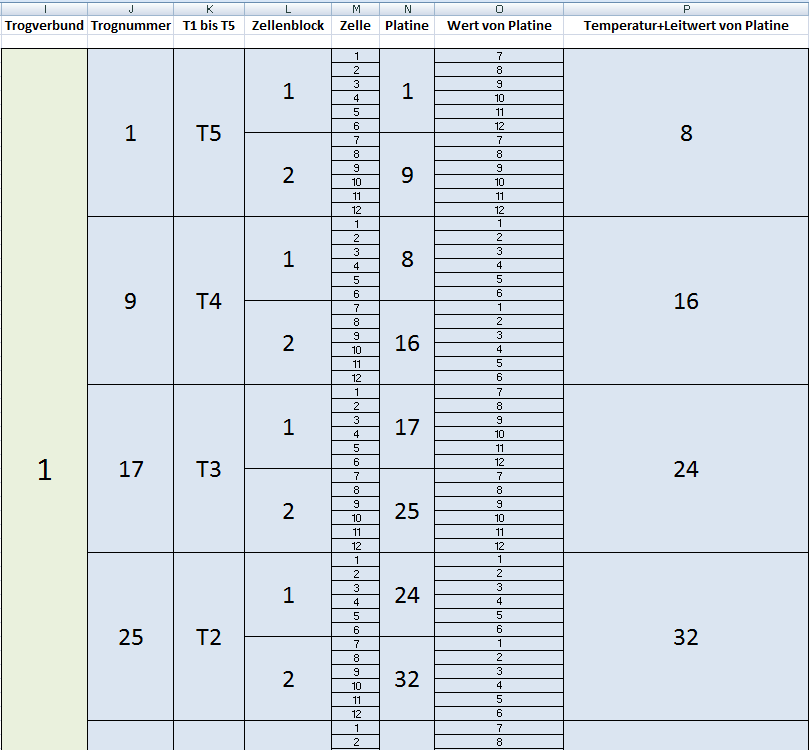
\includegraphics[width=0.42\textwidth]{images/example2_tabelle_excel.png}}
  \caption{Teil des �bersichtstabellen}
  \label{tabelle_excel}
\end{figure}

% Die Excel Tabellen erstellt, einen System gefunden, sehr viel Berechnen, logische Denken, Spannungswerten, Temperatur, Leitwert, Error

\begin{figure}[htbp]
  \centering
     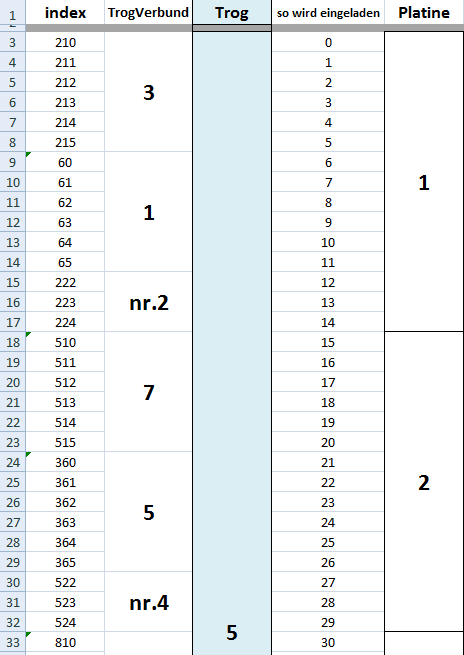
\includegraphics[width=0.9\textwidth]{images/example_tabelle_indexing.png}
  \caption{Tabelle mit Indexing}
  \label{example_tabelle_indexing}
\end{figure}

Nach dem die Fakten gesammelt wurden, kann man den Algorithmus entwickeln. Man muss die Zusammenh�nge finden und davon allgemeine Regeln bilden. Diese Regeln m�ssen alle Werte-Indexen beschreiben. Dann sind die Regeln zusammengefasst und wie m�glich es wird vereinfacht. Diese Vereinfachungen habe ich erstens mit Programmiersprache C beschreiben. Mit If- und Switch-Operatoren und for-Schleifen wurde die Zuordnung der jeweiligen Werte-Index auf die von uns feststellte Indexen durchgef�hrt. Man sollte den Algorithmus  

}\pagebreak

\section{Umwandlung in den \glqq Strukturierten Text\grqq \hspace{1mm}ST}
\large{(Damit es Johann implementieren kann, muss ich es in \textbf{ST} umwandeln, \textbf{ST} Syntax lernen, Die Implementierung)}


\section{Resultate}
\large{(Anwendung f�r die B\&R Steuerung, Screenshots von Johann)}